% Тут используется класс, установленный на сервере Papeeria. На случай, если
% текст понадобится редактировать где-то в другом месте, рядом лежит файл matmex-diploma-custom.cls
% который в момент своего создания был идентичен классу, установленному на сервере.
% Для того, чтобы им воспользоваться, замените matmex-diploma на matmex-diploma-custom
% Если вы работаете исключительно в Papeeria то мы настоятельно рекомендуем пользоваться
% классом matmex-diploma, поскольку он будет автоматически обновляться по мере внесения корректив
%

% По умолчанию используется шрифт 14 размера. Если нужен 12-й шрифт, уберите опцию [14pt]
\documentclass[14pt]{matmex-diploma}
%\documentclass[14pt]{matmex-diploma-custom}

\begin{document}
% Год, город, название университета и факультета предопределены,
% но можно и поменять.
% Если англоязычная титульная страница не нужна, то ее можно просто удалить.
\filltitle{ru}{
    chair              = {Кафедра Системного программирования},
    title              = {Разработка архитектуры для унификации синтаксических анализаторов в проекте YaccConstructor},
    % Здесь указывается тип работы. Возможные значения:
    %   coursework - Курсовая работа
    %   diploma - Диплом специалиста
    %   master - Диплом магистра
    %   bachelor - Диплом бакалавра
    type               = {coursework},
    position           = {студента},
    group              = 344,
    author             = {Соловьев Александр Александрович},
    supervisorPosition = {ст. преп., к.\,ф.-м.\,н.},
    supervisor         = {Григорьев С.\,В.}
}
\maketitle
\tableofcontents

\section*{Введение}
В области синтаксического анализа существует множество различных задач. Наиболее известной из них является задача анализа некоторой последовательности токенов с целью проверки ее выводимости в заданной грамматике и построением соответствующего дерева вывода. Однако данная задача может быть рассмотрена более широко, поскольку подвергаться синтаксическому анализу могут не только строки, но и другие структуры данных. Например, в работах \cite{graphParseVerb} и \cite{graphParseRag} в качестве объекта синтаксического анализа рассматривается граф.

В 2010 году был предложен алгоритм обобщенного синтаксического анализа Generalized LL (GLL), в основе которого лежит алгоритм нисходящего синтаксического анализа~\cite{GLLParsing}. Данный алгоритм и различные его модификации были реализованы в проекте YaccConstructor~\cite{YaccConstructor} независимо друг от друга (рис. \ref{fig:Old})). Различия их заключаются в первую очередь в структурах данных, которые подаются на вход, а также в возможности построения с помощью этих алгоритмов деревьев вывода. Конечно, отличается также и их внутренняя реализация, но общая структура различных версий при этом не меняется. Из сказанного выше следует, что поддерживать и сопровождать приходится все реализованные алгоритмы. Эту проблему могло бы решить их обобщение. Теоретически оно возможно, однако на практике возможно возникновение различных трудностей, получившееся решение может обладать рядом недостатков по сравнению с набором отдельно реализованных алгоритмов. Решение может быть крайне громоздким, что может еще больше усложнить его поддержку, одним же из наиболее вероятных недостатков, которые могут возникнуть, является значительное падение производительности. Например, при попытке представить линейный вход в виде графа, появляются циклы для перебора всех исходящих из вершины ребер, что приводит к увеличению числа операций.

\section{Постановка задачи}
Целью данной работы является разработка архитектуры для унификации существующих синтаксических анализаторов в проекте \newline YaccConstructor. Для достижения данной цели были поставлены следующие задачи:
\begin{itemize}
    \item спроектировать архитектуру, позволяющую объединить различные модификации алгоритма;
    \item реализовать предложенную архитектуру;
    \item разработать тестовое покрытие;
    \item провести эксперименты для оценки производительности.
\end{itemize}

\section{Обзор}
\subsection{YaccConstructor}
YaccConstructor --- проект, разрабатываемый в лаборатории языковых инструментов JetBrains, расположенной на кафедре системного программирования. В нем занимаются исследованиями и разработками в области лексического и синтаксического анализа. Большинство компонентов проекта реализованы на языке F\#, исходный код проекта находится в открытом доступе \cite{YaccConstructor}. Проект имеет модульную архитектуру (рис.\ref{fig:YCArch}), что позволяет собирать требуемый инструмент из существующих модулей: можно выбрать фронтенд, задать требуемые преобразования грамматики и указать генератор. Генераторы предоставляют инструменты, позволяющие по внутреннему представлению грамматики получить полезный для конечного пользователя результат. Примером такого результата являются синтаксические анализаторы.

\begin{figure}[h]
	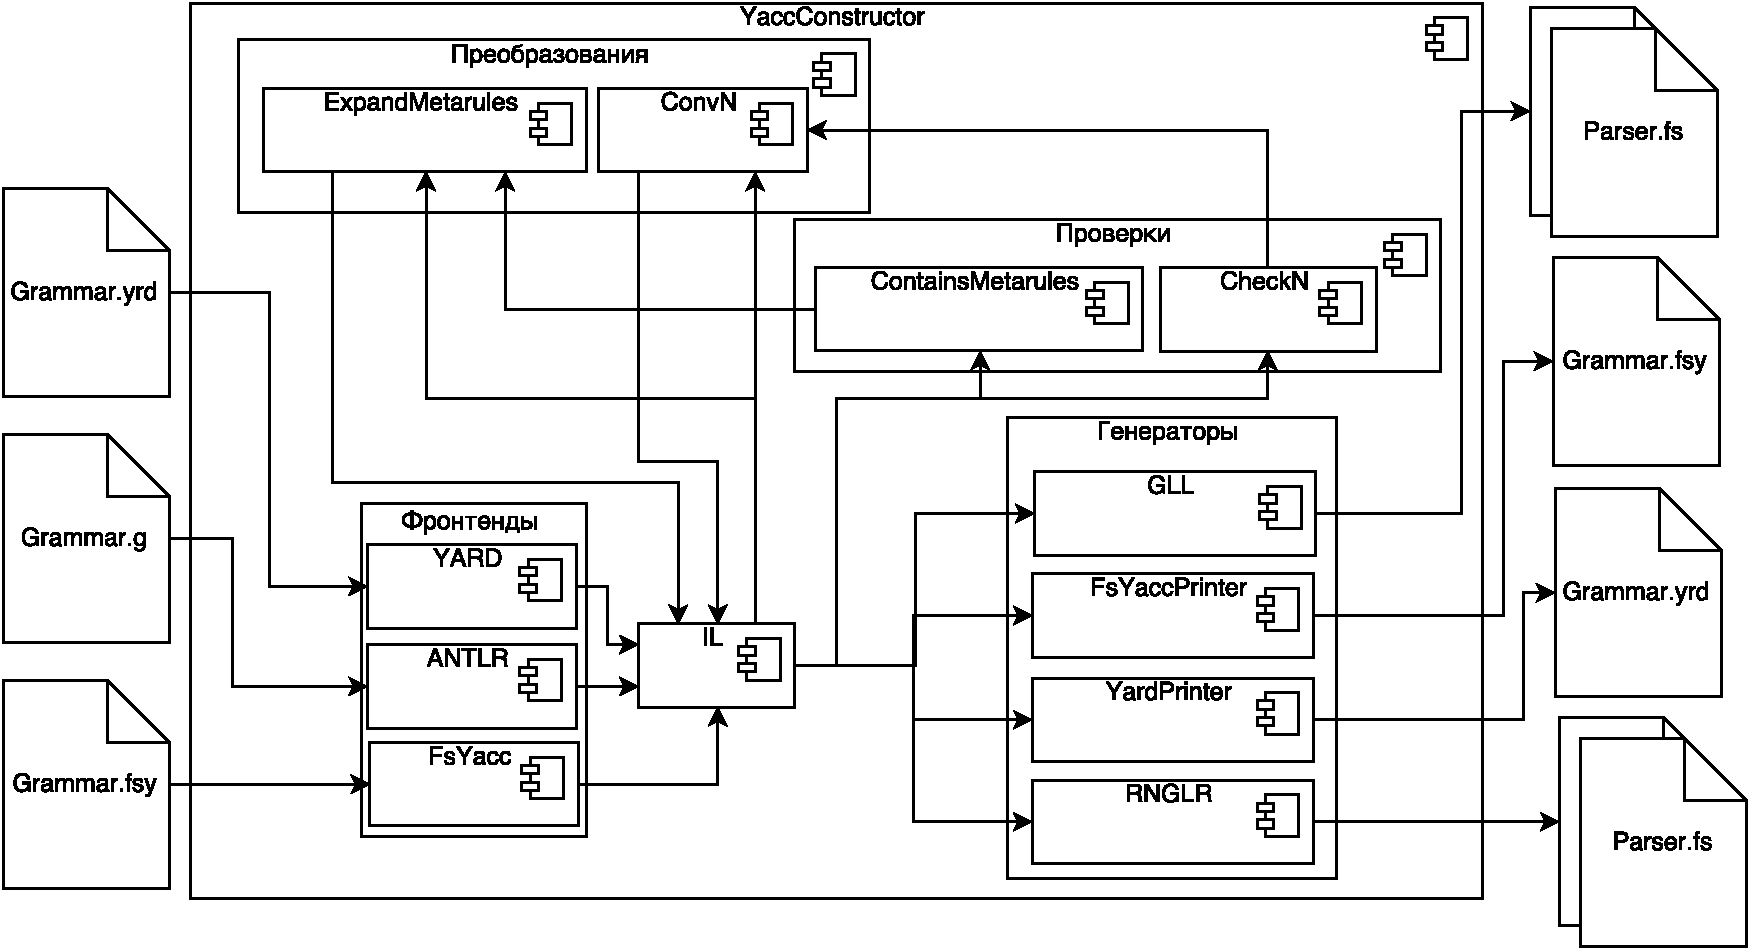
\includegraphics[width=\textwidth]{images/YCArch}
	\caption{Архитектура YaccConstructor, заимствована из \cite{gsvPhd}}
	\label{fig:YCArch}
\end{figure}

\subsection{Синтаксические анализаторы на основе GLL}
Как говорилось выше, на данный момент в проекте реализованы GLL и несколько его модификаций. Различаются они в рассматриваемой структуре данных, в возможности построения дерева вывода, а также в том, подается ли на вход алгоритму грамматика или же рекурсивный автомат \cite{RADesc}.

\subsubsection{Generalized LL}
GLL имеет некоторые преимущества перед прочими алгоритмами синтаксического анализа:
\begin{itemize}
    \item разбор любых контекстно-свободных грамматик, в том числе и неоднозначных;
    \item время исполнения в худшем случае кубически зависит от длины входной строки;
    \item алгоритм обладает свойством "рекурсивного спуска": анализатор может быть легко построен напрямую по грамматике.
\end{itemize}
Также, в 2013 году была представлена статья \cite{GLLTreeGen}, в которой описывалось построение дерева вывода при помощи GLL. В качестве дерева вывода в статье конструировалась структура SPPF (Shared Packed Parse Forest), представляющая все возможные выводы строки в заданной грамматике.

\subsubsection{Синтаксический анализ графов}
При решении различных практических задач может возникнуть необходимость проверки выводимости элементов некоторого регулярного множества в заданной грамматике. Если такое множество бесконечно, проверка всех его элементов на выводимость попросту невозможна. Однако, зачастую такие множества описываются при помощи конечных автоматов, таким образом задача сводится к проверке выводимости элементов, заданных конечным автоматом в заданной КС-грамматике. Примером подобной задачи может стать проверка корректности динамически формируемых SQL-запросов.

\subsubsection{Использование рекурсивного автомата}
\label{subsec:ra}
Процесс конструирования синтаксических анализаторов может быть автоматизирован при наличии требуемой спецификации с помощью генераторов. Подобным описание при этом может предоставляться в расширенной форме Бэкуса-Наура, справиться с которой способны немногие решения, при этом те из них, что способны, не умеют работать с неоднозначными грамматиками. Так в работе \cite{paperFSA} предлагается модификация GLL, позволяющая работать с грамматиками в форме, близкой к РФБН. Также показано, что данное решение имеет лучшую проивзодительность, чем при трансформации грамматики.

\subsection{Изначальная архитектура}
Как уже говорилось, основной проблемой данной архитектуры \ref{fig:Old} является проблематичность ее сопровждения, что является результатом целого ряда ее недостатков. Одним из самых серьезных недостатков является то, что используемые алгоритмами структуры данных, основными из которых являются GSS и SPPF, практически полностью реализуются отдельно для каждого алгоритма, причем различичя этих реализаций, как правило, незначительны. Некоторые структуры данных все же вынесены в прочие модули и используются несколькими реализациями сразу, но, как правило, для прочих реализаций существует практически такая же структура данных, исполняющая ту же роль в алгоритмах. Последнее приводит также и к тому, что при изменении такой общей структуры данных изменению также должны подвергнуться и использующие ее алгоритмы. Многое из сказанного выше распространяется также и на функции. 
Также проблематично расширение подобной архитектуры, ведь для некоторого нового алгоритма потребуется снова реализовывать многие структуры данных и функции, возможно, будет иметься необходимость в реализации сразу нескольких версий алгоритма, например, для разных представлений грамматики.
\begin{figure}[h]
    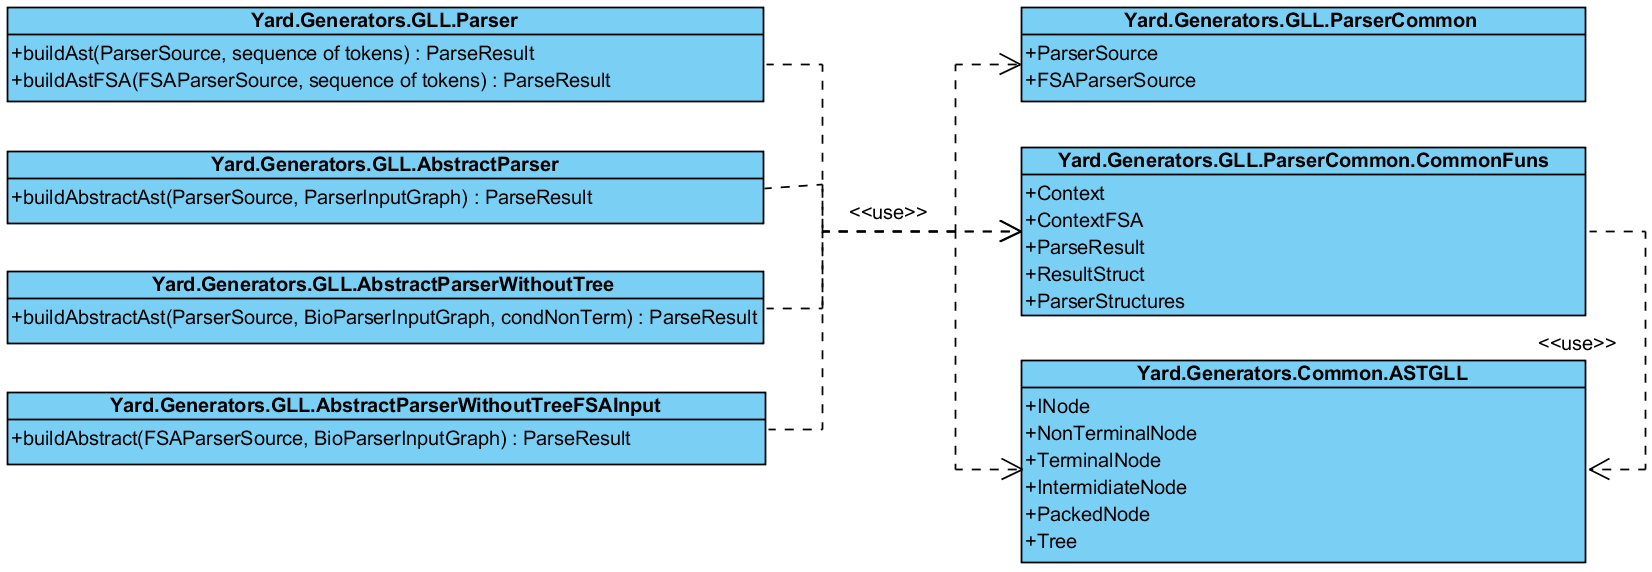
\includegraphics[width=\textwidth]{images/Old}
    \caption{Взаимодействие основных модулей при изначальной архитектуре}
    \label{fig:Old}
\end{figure}

\section{Предложенная архитекура}
Предложенное решение позволяет избежать упоямнутых ранее проблем. В связи с тем, что различия в действии над входными данными зависят исключительно от их внутреннего представления, было решено использовать некоторую абстракцию, конкретные реализации которой ответственны за эти различия. Подобное решение позволяет обобщить алгоритм для различных входных данных. Также было решено в качестве представления грамматики использовать рекурсивный автомат из-за его достоинств, которые были описаны в разделе \ref{subsec:ra}. Структуры GSS (Graph Structured Stack) и SPPF в свою очередь были выделены в отдельные сущности, что приводит к снятию с алгоритма ответственности за работу с ними. Различие в построении дерева релазиуется через передаваемый алгоритму флаг, что позволяет строить дерево лишь, когда оно нужно пользователю. Таким образом остается только одна версия алгоритма, обобщенная для входной грамматики и представления входных данных и умеющая строить дерево при необходимости.
\begin{figure}[h]
    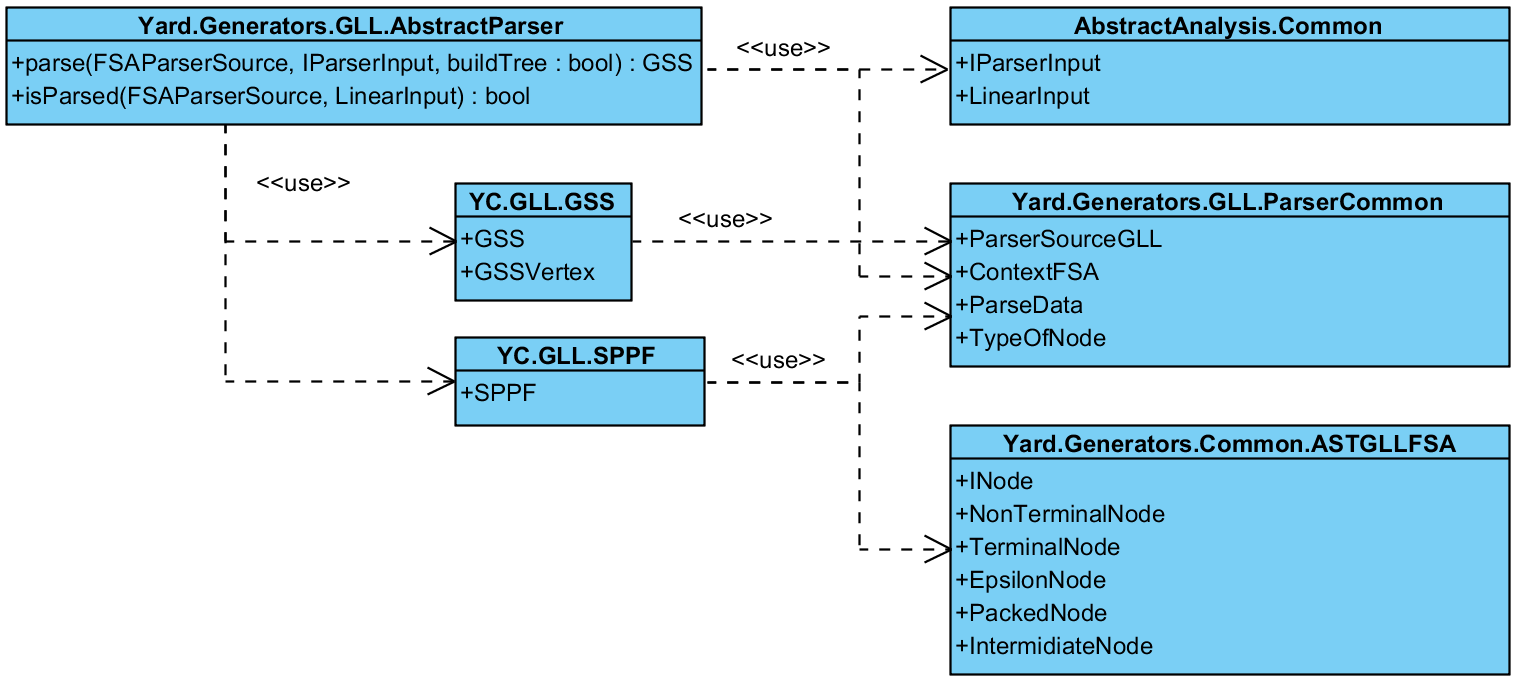
\includegraphics[width=\textwidth]{images/New}
    \caption{Архитектура решения после унификации}
    \label{fig:New}
\end{figure}

\section{Заключение}
Достигнуты следующие результаты:
\begin{itemize}
    \item произведен обзор статей, связанных с предметной областью;
    \item написан обзор предметной области;
    \item спроектирована и реализована архитектура (рис. \ref{fig:New}).
\end{itemize}
В дальнейшем планируется:
\begin{itemize}
    \item написать докумментацию;
    \item разработать тестовое покрытие;
    \item провести эксперименты для оценки производительности.
\end{itemize}

\setmonofont[Mapping=tex-text]{CMU Typewriter Text}
\bibliographystyle{ugost2008ls}
\bibliography{diploma.bib}
\end{document}
